\chapter{Systemarchitektur}
\label{chap:systemarchitektur}

Aufbauend auf den Systemanforderungen in Kapitel \ref{chap:systemanforderungen} wird in diesem Kapitel der Entwurf der Systemarchitektur beschrieben. Da eine als Couchapp umgesetzte Anwendung eine Architektur ohne Middleware ermöglicht, liegt der Schwerpunkt weniger auf der Darstellung der Komponenten. Stattdessen wird die innere Struktur der Anwendung vorgestellt. Die in Frage kommenden Konzepte für die zentralen Problemstellungen bei der Konzeption werden diskutiert und die jeweils getroffene Wahl begründet. So wird ein Überblick über die Funktionsweise der Datenhaltung, der Anwendungslogik sowie der Benutzeroberfläche vermittelt.

Die Code-Beispiele in diesem Kapitel sind nicht die kompletten CouchDB-Dokumente. Sie enthalten lediglich die Teile, die für die Demonstration der jeweiligen Aspekte wichtig sind.



\section{Gesamtüberblick über die Architektur}

Klassische Webanwendungen sind nach der \textit{Client-Server}-Architektur aufgebaut: Die Daten liegen in einer meist relationalen Datenbank, die Anwendungslogik wird auf dem Server ausgeführt und die Ergebnisse werden an den Client ausgeliefert (s. Abb. \ref{fig:old-web-arch}). Lediglich kleine Teile der Darstellungslogik werden manchmal als \textit{Add-On} im Webbrowser abgearbeitet, um die Anwenderakzeptanz zu verbessern.


\medskip
\begin{figure}[ht] 
  \begin{center}
    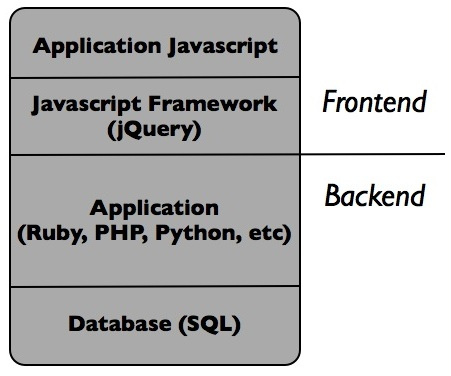
\includegraphics[width=0.5\textwidth]{grafik/old-application-architecture} 
  \end{center}
\caption{Architektur einer klassischen Webanwendung, nach \cite{web:architecture}}
\label{fig:old-web-arch} 
\end{figure}


Setzt man nun voraus, dass der Browser JavaScript und HTML5 unterstützt, können auch größere Teile der Applikation lokal auf dem Rechner des Benutzers ausgeführt werden. CouchDB bringt darüber hinaus einen eigenen Webserver mit. Dadurch entfällt die Notwendigkeit, für die Applikationslogik eine Middleware zu erstellen (s. Abb. \ref{fig:new-web-arch}).

\medskip
\begin{figure}[ht] 
  \begin{center}
    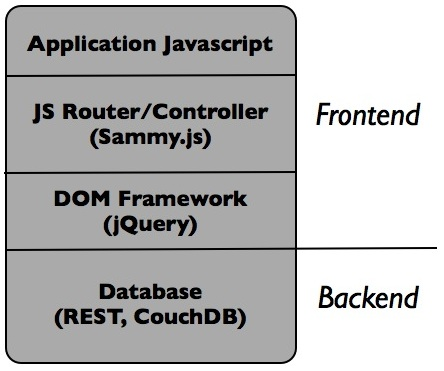
\includegraphics[width=0.5\textwidth]{grafik/new-application-architecture} 
  \end{center}
\caption{Architektur einer Couchapp, nach \cite{web:architecture}}
\label{fig:new-web-arch} 
\end{figure}

\afterpage{\clearpage}

Ist CouchDB auf dem lokalen Rechner installiert, kann die Anwendung wie ein Desktop-Programm benutzt werden. Die Instanz auf dem Server dient lediglich dazu, die Outlines zwischen den Clients zu synchronisieren (s. Abb.
\ref{fig:projektvision}). Es reicht aus, eine einzige Anwendung zu implementieren, die auf den Clients sowie auf dem Server eingesetzt wird. Auf den Clients kann die Anwendung auch eingesetzt werden, wenn der Server nicht erreichbar ist.

\medskip
\begin{figure}[H] 
  \begin{center}
    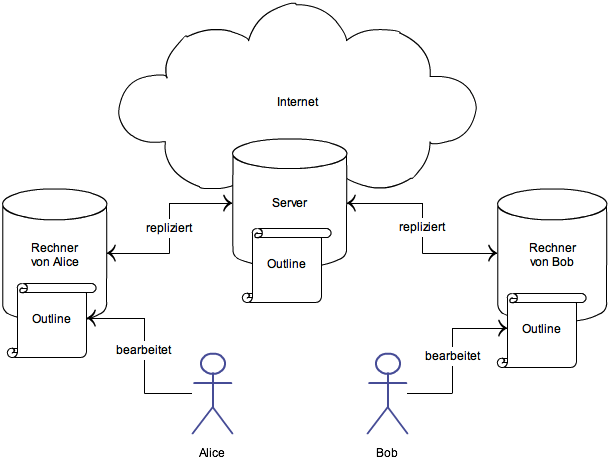
\includegraphics[width=0.85\textwidth]{grafik/Projektvision} 
  \end{center}
  \caption{Projektvision}
  \label{fig:projektvision} 
\end{figure}


\section{Modellierung der Datenstruktur}

Für die Abbildung der Daten in der Datenbank kamen mehrere Alternativen in Frage. Durch die Diskussion dieser Möglichkeiten wird die gewählte Lösung begründet.

\subsection{Anforderungen}
\label{subsec:ana-anf}

Die Anforderungen an den Entwurf der Datenmodellierung werden in folgender Priorität definiert:

\begin{itemize}
  \item Die Programmierung und Wartung der Anwendung soll möglichst einfach sein.
  \item Konflikte beim gleichzeitigen Speichern von Daten sollen möglichst vermieden werden oder nur selten auftreten. 
  \item Der Zugriff auf die Daten soll möglichst performant sein. Da weniger Abfragen zu kürzeren Zugriffszeiten führen, sollen die zusammengehörenden Daten möglichst auch zusammen gespeichert werden. 
\end{itemize}

CouchDB ermöglicht eine Replikation, bei der konflikthafte Dokumente automatisch markiert werden. Für eine benutzbare Anwendung muss jedoch eine Anwendungslogik umgesetzt werden, die die Auflösung dieser Konflikte ermöglicht. Für den Entwurf der Datenstruktur wurden Hinweise aus \cite{design:replication} entnommen.

\subsection{Problemstellung}

Ein Outline ist eine sortierte, hierarchisch verschachtelte Liste von unterschiedlich tief eingerückten Zeilen. Ein einfaches Beispiel findet sich in Abbildung \ref{fig:nestedoutline}. Dabei sind die Aufzählungszeichen für Zeilen ohne Kindknoten Kreise, für Zeilen mit Kindknoten Dreiecke. Ein solches Outline soll möglichst entsprechend der oben genannten Anforderungen umgesetzt werden.

Im Beispiel wird mithilfe des Outliners eine Einkaufsliste umgesetzt. Dies stellt sicher nicht den zentralen Anwendungsfall für einen Gliederungseditor dar; dafür wird die hierarchische Einrückung intuitiv deutlich, und das Beispiel kann kurz, aber realistisch gehalten werden.
 
\medskip
\begin{figure}[ht] 
  \begin{center}
    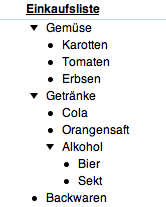
\includegraphics[width=0.3\textwidth]{grafik/nested-outline} 
  \end{center}
  \caption{Einfaches Outline}
  \label{fig:nestedoutline}
\end{figure}

\subsection{Speicherung in einem JSON-Dokument}

Die einfachste Implementierung ist die Umsetzung in einem einzigen JSON-Dokument (s. Listing \ref{lst:nestedoutline}). Bei diesem Entwurf müssen die Zeilen wiederum eigene JSON-Objekte sein, damit sie geschachtelt gespeichert werden können. 


Von diesem Outline werden während der Lebensdauer der Anwendung zeitweise zwei (oder mehr) Versionen existieren, die sich voneinander unterscheiden. Bei der nächsten Synchronisierung der beiden Versionen sollen diese wieder zusammengeführt werden. Zeilen, die verändert, hinzugefügt oder gelöscht werden, sollen auch in der anderen Version verändert, hinzugefügt oder gelöscht werden. Der Benutzer muss nur intervenieren, wenn für dieselbe Zeile zwei konkurrierende Versionen vorliegen. Wie kann dies erreicht werden?

\medskip
\begin{lstlisting}[caption=Einfaches Outline in einem JSON-Dokument, label={lst:nestedoutline}]
{
  "title": "Einkaufsliste",
  "lines": [
    {"text": "Gemüse", "lines": [
      {"text": "Karotten"},
      {"text": "Tomaten"}, 
      {"text": "Erbsen"}
    ]}, 
    {"text": "Getränke", "lines": [
      {"text": "Cola"},
      {"text": "Orangensaft"}, 
      {"text": "Alkohol", "lines": [
        {"text": "Bier"},
        {"text": "Sekt"}
      ]},
    ]},
    {"text": "Backwaren"}
  ]
}
\end{lstlisting}




Die Struktur in Listing \ref{lst:nestedoutline} ist bereits valides JSON. In CouchDB könnte es in dieser Form in einem einzigen Dokument gespeichert werden. Dieses Dokument könnte dann mit einem einzigen Lesezugriff gelesen werden. Für die Replikation wird ebenfalls nur ein einziger Vorgang benötigt. Auch die Umsetzung der Anwendungslogik ist vergleichsweise simpel, da die für das Sortieren und das Einrücken der Zeilen nötigen Informationen schon im Dokument enthalten sind.

Probleme treten jedoch auf, sobald das Dokument modifiziert wird. Wenn eine Zeile verändert, hinzugefügt oder verschoben wird, speichert CouchDB für das Outline-Dokument eine neue Version mit einer neuen Revisionsnummer. Ein Konflikt entsteht ausnahmslos jedesmal, wenn das Outline nach der Modifikation mit der Version eines anderen Benutzers repliziert wird. 

Auch nach einer Replikation mit vielen Änderungen im Dokument gibt es nur zwei verschiedene Sets von Zeilen. Ein Set wird als die Gewinner-Revision, das andere als die konflikthafte Revision gespeichert werden. Diese Semantik ist sehr unpraktisch für den Benutzer: Er kann nur noch seine eigene oder die andere Version zum Behalten auswählen. So müssen sämtliche Änderungen wieder manuell angewendet werden. Zentrale Vorteile der CouchDB-Replikation sind somit verfallen. 

\subsection{System Prevalence}

Eine weitere Möglichkeit der Umsetzung ist die Anwendung von \textit{System Prevalence} \cite{prevalence}. Diese Persistierungstechnik wird in Objektdatenbanken wie Madeleine \cite{madeleine} angewandt. Anstatt neuer Versionen des Outlines werden Operationen auf einem Ausgangsdatensatz gespeichert. So sind \enquote{Ändern}, \enquote{Speichern}, \enquote{Verschieben} einer Zeile einzelne Einträge in der Geschichte des Outlines. Diese Einträge werden nacheinander gespeichert und nie verändert. So entstehen niemals Konflikte bei der Replikation. Die Einträge können in einem Array in einem einzelnen CouchDB-Dokument gespeichert werden. Wenn bei der Replikation Konflikte auftreten, sind diese leicht zu lösen, indem die Elemente der beiden Arrays kombiniert werden.

Probleme treten auch hier auf, denn wenn unterschiedliche Versionen zusammengeführt werden, hat die Reihenfolge der Änderungen Auswirkungen auf das Ergebnis. Es müsste ein Algorithmus entwickelt werden, der die Reihenfolge der Änderungen sinnvoll festlegt.


\subsection{Speicherung der Versionshistorie}

Anstatt die Historie der Kommandos zu speichern, könnten auch die alten Revisionen der Outlines gespeichert werden. CouchDB löscht alte Revisionen nach einem {\fontfamily{pcr}\selectfont compact}-Vorgang der Datenbank. Um dies zu verhindern, könnten die Revisionen in eigene Dokumente persistiert werden. Das System muss eine Referenz auf die aktuellste Revision speichern, jede Revision muss auf ihren Vorgänger verweisen. Beim Zusammenführen nach einem Replikationsvorgang könnten die abweichenden Versionen so lange verglichen werden, bis der letzte gemeinsame Vorgänger gefunden ist. Auf dieser Basis kann dann das Zusammenführen stattfinden.

Dieses Verfahren wird von Versionskontrollsystemen wie Git oder Subversion angewendet. Hier müssten entsprechend JSON-Felder anstelle von Zeilen innerhalb von Textdateien verglichen werden.  

Mit dieser Vorgehensweise wird also für jeden Schreibvorgang eine komplette Version des gesamten Outlines gespeichert. Dabei steigt der Umfang der Daten in der Datenbank stark an. Dies ist ein beträchtlicher Nachteil. Beim Zusammenführen müssen anwendungsseitig beide Versionen der Dokumente zerlegt werden, um feststellen zu können, in welcher Version welche Zeile auf welche Weise verändert wurde. Dieses Vorgehen wurde mithilfe eines einfachen Prototypen mit geringem Funktionsumfang getestet, jedoch schnell als zu komplex verworfen. Stattdessen sollte ein Verfahren entwickelt werden, bei dem die Zerlegung schon im Dokument vorgenommen wird, um das Qualitätsziel der möglichst geringen Komplexität zu beachten.

\subsection{Ausgliedern der Zeilen in einzelne JSON-Dokumente}

Die letzte untersuchte Möglichkeit ist, jede Zeile in einem eigenen Dokument zu speichern. Das Hinzufügen oder Löschen einer Zeile wird über das Erstellen oder Löschen eines JSON-Dokumentes umgesetzt. Aus diesem Vorgang entsteht nicht per se ein Konflikt. Das Ändern einer Zeile wird nur dann zu einem Konflikt führen, wenn beide Seiten gleichzeitig dieselbe Zeile verändern. Erst diese Situation erfordert die Intervention eines Benutzers. Das Thema der Replikation ist so relativ trivial in der Anwendung zu lösen. 

Aus dieser Art, das Problem zu modellieren, resultieren viele kleine Dokumente in der Datenbank, die jeweils nur eine Zeile enthalten. Deswegen muss ein Attribut eingeführt werden, mit dem Zeilen von Outlines in der Datenbank unterschieden werden können. Jedes Zeilen-Dokument enthält eine Referenz auf das Outline, zu dem es gehört. 

Mit dieser Herangehensweise ergibt sich das Problem, dass die Sortierung und die Schachtelung der Zeilen nicht mehr innerhalb des Dokumentes persisiert sind. Die Lösung für dieses Problem wird in Abschnitt \ref{sec:sortierung} eigens behandelt. 

\subsection{Fazit}
\label{subsec:viewabfrage}

Alle vier Lösungen haben gemeinsam, dass die Historie der Daten in irgendeiner Form gespeichert werden muss, denn nur so kann beim Zusammenführen der Repliken der aktuelle Zustand der Daten mit dem Zustand verglichen werden, in dem sich die Versionen noch nicht unterschieden haben. CouchDB speichert verschiedene Versionen von Dokumenten; es ist sinnvoll, sich dieses Feature zunutze zu machen. Der einfachste und am wenigsten fehleranfällige Weg ist daher, die Zeilen als eigene Dokumente zu speichern. Dies wird in Listings \ref{lst:outlineforview} und \ref{lst:linesforview} beispielhaft dargestellt.


\medskip
\begin{lstlisting}[caption=Outline mit ID und Typ, label={lst:outlineforview}]
{
  "_id": "1dbdcbc27b22cc7a14cd48d397000657",
  "kind": "Outline",
  "title": "Einkaufsliste"
}
\end{lstlisting}

\medskip
\begin{lstlisting}[caption=Drei Zeilen mit ID und Typ, label={lst:linesforview}]
{
   "kind": "Line",
   "text": "Gemüse",
   "outline_id": "1dbdcbc27b22cc7a14cd48d397000657"
},
{
   "kind": "Line",
   "text": "Getränke",
   "outline_id": "1dbdcbc27b22cc7a14cd48d397000657"
},
{
   "kind": "Line",
   "text": "Backwaren",
   "outline_id": "1dbdcbc27b22cc7a14cd48d397000657"
}
\end{lstlisting}

Durch die Erstellung einer CouchDB-View mit einem zusammengesetzten Schlüssel können Outline und alle ihre Zeilen in nur einem Request abgefragt werden. Für dieses Problem wird die weit verbreitete Technik der \textit{View-Collation} eingesetzt, die das Bilden von Joins simuliert \cite{couchdb:joins}. Mehr zum Einsatz von Views siehe \ref{subsec:views}. Der Schlüssel dieser View ist ein JSON-Array, dass sich aus der Outline-ID und einer Zahl zusammensetzt. Die Zahl ist bei Dokumenten mit Typ {\fontfamily{pcr}\selectfont Outline} eine 0, bei Dokumenten mit Typ {\fontfamily{pcr}\selectfont Line} eine 1. Da die Schlüssel die Kollation (für die Sortierreihenfolge) der Zeilen beeinflussen, wird das erste Element des resultierenden Arrays immer das Outline sein. Erst darauf folgen alle Zeilen. Das Dokument ist der Value eines jeden Array-Elements. Mit diesem definierten Ergebnis kann nun die Anwendung die Ausgabe eines Outlines mit allen zugehörigen Zeilen vornehmen.

Die View ist in Listing \ref{lst:viewnotesbyoutline} angegeben. Abgefragt wird sie mit der Outline-ID als Key-Parameter. Dadurch werden nur dieses Outline und die zugehörigen Zeilen ausgegeben: \url{http://localhost:5984/doingnotes/_design/doingnotes/_view/notes_by_outline?key="01234567890"}. Im diesem Beispiel hat das Outline die ID \enquote{01234567890}. 

\medskip
\begin{lstlisting}[caption=View zum Ausgeben aller Zeilen zu einem Outline, label={lst:viewnotesbyoutline}]
function(doc) {
  if (doc.kind == "Outline") {
    emit([doc._id, 0], doc);
  } else if (doc.kind == "Line") {
    emit([doc.outline_id, 1], doc);
  }
}
\end{lstlisting}

Nachdem die Entscheidung für den Ansatz der Datenmodellierung getroffen wurde, bleibt das Problem zu lösen, wie Sortierung und Einrückung der Zeilen am besten abzubilden sind. Dies wird im nächsten Abschnitt diskutiert.


\section{Umsetzung der Zeilensortierung und -einrückung}
\label{sec:sortierung}

Es muss ein im Bezug auf die in Abschnitt \ref{subsec:ana-anf} genannten Anforderungen effektiver Weg gefunden werden, wie Reihenfolge und Einrückungsgrad der Zeilen in einem Outline gespeichert werden können. Das Ziel ist die Abbildung der in Abbildung \ref{fig:nestedoutline} beschriebenen Struktur. Mehrere Möglichkeiten, dieses Problem zu lösen, sind denkbar. Es ist zu unterscheiden, ob es vorteilhafter ist, die Zeilen zu verbinden, sei es in Form einer verketteten Liste oder als Baumstruktur, oder ob es praktikabler ist, die Sortierreihenfolge in den Zeilen festzulegen. In diesem Abschnitt werden die Vor- und Nachteile für beide Ansätze abgewogen. 

Die Anforderungen an die Lösung sind, dass das Einfügen, Löschen und Verschieben einer Zeile mit möglichst wenig Schreibzugriffen verbunden ist. Außerdem soll die Position einer Zeile immer genau definiert sein; Zeilen dürfen weder denselben Platz beanspruchen, noch darf die Information über ihre Positionierung verlorengehen.


\subsection{Indiziertes Array}
\label{subsec:array}

Der erste untersuchte Ansatz ist, die Zeilen als ungeordnete Liste zu speichern und ihnen einen Index zuzuweisen. Die Information über den Grad der Einrückung muss bei dieser Vorgehensweise ebenfalls explizit gespeichert werden.

\subsubsection{Sortierung}

Listing \ref{lst:sortOutlineLines} ist ein Beispiel für den Einsatz von Sort-IDs.

\medskip
\begin{lstlisting}[caption=Drei Zeilen mit einfachem Index, label={lst:sortOutlineLines}]
{
  "text": "Gemüse",
  "sort_id": "1"
},
{
  "text": "Getränke",
  "sort_id": "2"
},
{
  "text": "Backwaren",
  "sort_id": "3"
}
\end{lstlisting}

Wenn nun ein Element eingefügt wird, erhält das Element die  {\fontfamily{pcr}\selectfont Sort-ID} des nachfolgenden Elements, und jedem der nachfolgenden Elemente muss ein neuer Index zugewiesen werden. Dies ist problematisch, weil die Anzahl der Schreibzugriffe bei zunehmender Länge des Dokuments sehr schnell ansteigt. Die trivialste Lösung wäre, Indizes mit sehr hohem Abstand zu vergeben (0, 1000, 2000). Dies ist jedoch kein skalierbarer Ansatz: Im ungünstigsten Fall müssen Indizes sehr schnell mehrfach zugewiesen werden, wenn mehrere Elemente an derselben Stelle eingefügt werden. 

Eine andere Möglichkeit ist es, für den Index den Datentyp \textit{Floating Point} zu wählen. Dieser Ansatz wird in \citelit[Kap. 24]{couchdb} vorgeschlagen. Beim Einfügen erhält ein Element als Index den Mittelwert zwischen den Indizes der beiden umgebenden Elemente. Am Beispiel von Listing \ref{lst:floatsortOutlineLines}: Wird eine Zeile zwischen {\fontfamily{pcr}\selectfont Gemüse} und {\fontfamily{pcr}\selectfont Getränke} eingefügt, erhält sie als Index $\frac{(0.2 + 0.3)}{2} = \frac{0.5}{2} = 0.25$.


\medskip
\begin{lstlisting}[caption=Drei Zeilen mit Float-Index, label={lst:floatsortOutlineLines}]
{
  "text": "Gemüse",
  "sort_id": 0.1
},
{
  "text": "Getränke",
  "sort_id": 0.2
},
{
  "text": "Backwaren",
  "sort_id": 0.3
}
\end{lstlisting}

Der Vorteil dieser Herangehensweise ist, dass für Verschieben und Einfügen einer Zeile nur ein einziger Schreibzugriff notwendig ist.

Das Problem an diesem Ansatz ist, dass die Präzision des Datentyps Float begrenzt ist. Bei häufigem Verschieben der Zeilen würde die maximale Anzahl der Nachkommastellen schnell erreicht werden. Indizes würden wieder mehrfach vergeben, wenn die Anzahl der Zeilen eines Outlines ansteigt. Dies könnte mit einem regelmäßigen Zurücksetzen der Indizes auf Zahlen mit geringerer Anzahl Stellen verhindert werden. Dies ist für ein verteiltes Setup jedoch nicht praktikabel, da bei dem Zurücksetzen alle anderen Benutzer einen Hinweis auf Änderungen im gesamten Outline erhalten würden. Darüber hinaus würden durch diese Operation zahlreiche Konflikte entstehen.

In \cite{design:replication} wird empfohlen, den Index als String zu implementieren, dem bei jedem Verschieben ein Zeichen hinzugefügt wird. So umgeht man das Problem der Float-Präzision. Allerdings würde die Länge der Strings mit der Zeit ebenfalls stark ansteigen, was am Ende zu einem ähnlichen Problem wie bei der Umsetzung mit Floating Points führen würde.

Der Vorteil beider Herangehensweisen ist, dass für Verschieben und Einfügen einer Zeile nur ein einziger Schreibzugriff notwendig ist.

\subsubsection{Einrückung}
\label{subsec:einrueckung}

Sind die Zeilen nun in einer sortierten Liste gespeichert, müssen sie noch mit Information über den Grad der Einrückung versehen werden. Beim Ausgeben des Outlines wird diese Information ins DOM übertragen. 

Dafür gibt es zwei Ansätze. Eine Zeile erhält entweder ein Attribut mit der Information, wie weit sie eingerückt ist (\lstinline!"indent": 0, "indent": 1, "indent": 2!). Oder ihre Einrückungsdifferenz nach oben wird als Zahl gespeichert (\lstinline!"indent": 0, "indent": 1, "indent": -1!). Der letztere Ansatz hat den Nachteil, dass beim Einrücken einer Zeile alle nachfolgenden Zeilen verändert werden müssen.

Der Nachteil beider Herangehensweisen ist, dass beim Ein- bzw. Ausrücken einer Zeile die unmittelbar darunter liegenden Zeilen mit tieferer bzw. gleicher Einrückung mitbewegt werden sollen. Für alle diese Zeilen muss dann ebenfalls ein eigener Schreibzugriff stattfinden. Je nach Beschaffenheit des Outlines kann die Anzahl der Schreibzugriffe stark ansteigen.


\subsection{Verkettete Liste}

Eine Alternative zur Umsetzung als indiziertes Array ist eine einfach verkettete Liste. Eine verkettete Liste ist eine Datenstruktur, in der die Objekte linear angeordnet sind. Im Gegensatz zu einem Array, bei dem die Reihenfolge von den Array-Indizes bestimmt wird, wird die Reihenfolge in einer verketteten Liste von Zeigern in jedem Objekt bestimmt \citelit[Kap. 10.2]{algorithms}. 

Bei diesem Ansatz entfällt das Problem mit der (Neu-)Vergabe der Indizes beim Verschieben oder Einfügen von Elementen. Das Einfügen einer Zeile erfordert zwar einen Schreibzugriff zusätzlich zum Speichern der Zeile, da der neue Vorgänger seinen Zeiger auf die Zeile richten muss. Dies ist aber die maximale Anzahl der Schreibzugriffe, unabhängig von Komplexität und Länge des Outlines. Das Verschieben einer Zeile kann ebenfalls mit maximal zwei Schreibzugriffen umgesetzt werden. 

Allerdings muss bei diesem Weg die Einrückung einer Zeile genauso umgesetzt werden wie bei der Umsetzung als indiziertes Array (s. Abschnitt \ref{subsec:einrueckung}). Die Nachteile bei den beschriebenen Lösungsansätzen hierfür bleiben bestehen.


\subsection{Baumstruktur}

\subsubsection{Terminologie}

Als Argument für die Modellierung als Baumstruktur sind die oben genannten Nachteile insbesondere bei der Einrückung einer sortierten Liste zu nennen. Baumstrukturen gehören zu den wichtigsten Datenstrukturen der Informatik. 
Laut \citelit{knuth} handelt es sich um die wichtigsten nichtlinearen Strukturen unter den Computer-Algorithmen. Den Erfinder dieser Datenstruktur festzustellen ist nicht möglich \citelit[S. 89]{datenstrukturen}. Als Baumstruktur wird generell eine \enquote{verästelte} Beziehung zwischen Knoten bezeichnet. 

Die Terminologie für Elemente von Bäumen ist in der Literatur nicht einheitlich. In \citelit{knuth} werden folgende Bezeichnungen verwendet: Jede Wurzel ist \textit{Elternknoten (parent)} von den Wurzeln der Teilbäume. Unmittelbar benachbarte Knoten sind untereinander \textit{Geschwister (siblings)}, und \textit{Kinder (children)} ihrer Eltern. Außerdem werden die Begriffe \textit{Vorgänger (ancestor)} und \textit{Nachkomme (descendant)} eingesetzt, um eine Beziehung zu beschreiben, die mehrere Ebenen eines Baums umspannt. 

Laut der Klassizierung in \citelit[Kap. 2.3.4]{knuth} handelt es sich bei dem hier eingesetzten Baum um einen \textit{Finite labeled rooted ordered Tree}. Jeder Knoten muss dabei einen Elternknoten haben; der Knoten ohne Elternknoten wird als Wurzel bezeichnet. Zyklische Beziehungen sind nicht erlaubt; vom Wurzelknoten aus ist jeder Knoten durch genau einen gerichteten Pfad erreichbar.

\subsubsection{Umsetzung}
\label{subsec:baumumsetzung}

In \citelit[Kap. 10.4]{algorithms}, werden Verfahren vorgestellt, wie eine Baumstruktur mithilfe von Zeigern umgesetzt werden kann. Das für das vorliegende Problem am besten geeignete Verfahren wird hier beschrieben. Es handelt sich um die \textit{left child, right sibling}-Repräsentierung. Jeder Knoten ist dabei durch eine ID identifiziert. Jeder Knoten enthält einen Zeiger zu seinem ganz linken Kind, dem in einer vertikalen Abbildungsweise mit der Wurzel oben dem ersten Kind entspricht, und einen Zeiger zu seinem rechten Geschwisterknoten, also zu dem in der gleichen Ebene liegenden nächsten Knoten.

Der Vorteil an diesem Verfahren ist, dass die Anzahl der Schreibzugriffe bei jeder Art Operation zwei nicht übersteigt. Dies schließt das Ein- und Ausrücken eines ganzen Zeilenblocks mit ein.  

\subsection{Fazit}

Nach Abwägen der Vor- und Nachteile wurde entschieden, die Anwendung mit einer Baumstruktur umzusetzen. Die konstante Anzahl der Schreibzugriffe beim Einsatz dieser Datenstruktur gab den Ausschlag.

Mit einer View können ein Outline und alle zugehörigen Outlines auf einmal abgerufen werden, dies wurde bereits in Abschnitt \ref{subsec:viewabfrage} skizziert. Es ist ein für die Anwendung gewünschtes Verhalten, dass dies auf einmal geschieht. Die Zeilen werden nicht etwa erst bei Bedarf geladen, z.\,B. beim Ausklappen der Zeilen. Wie in Abschnitt \ref{subsec:gliederungseditor} spezifiziert, soll der Outliner einem Texteditor ähneln, bei dem man auf den ersten Blick das gesamte Dokument erfassen kann und nur bei Bedarf einzelne Abschnitte verbirgt. Für die Ausgabe der Zeilen eines Outlines muss eine rekursive Funktion implementiert werden.

Mit einer leichten Abwandlung soll das Verfahren eingesetzt werden, das in Abschnitt \ref{subsec:baumumsetzung} zuletzt beschrieben wurde. Jeder Knoten enthält statt eines Zeigers zu seinem ersten Kind einen Zeiger zu seinem Elternknoten. So muss beim Ein- oder Ausrücken einer Zeile nur der ein- oder ausgerückte Knoten verändert werden, der neue Elternknoten bleibt unverändert. Die Zeigerstruktur sieht demnach aus wie in Abbildung \ref{fig:pointer}. 

\medskip
\begin{figure}[H] 
  \begin{center}
    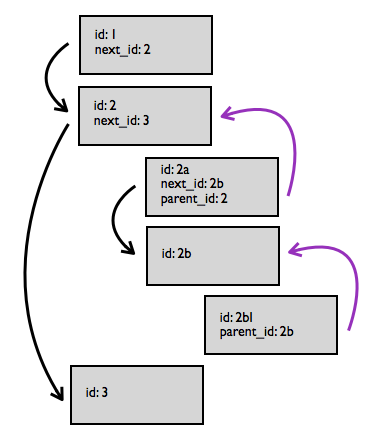
\includegraphics[width=0.6\textwidth]{grafik/pointer} 
  \end{center}
  \caption{Die Zeiger-Struktur}
  \label{fig:pointer}
\end{figure}


Mit dem Umsetzen der Zeigerstruktur sieht das Beispiel-Outline aus Abbildung \ref{fig:nestedoutline} am Ende aus wie in den Listings \ref{lst:theoutline} und \ref{lst:outlineLines}. 

\medskip
\begin{lstlisting}[caption=Gewählte Implementierung eines Outlines, label={lst:theoutline}]
{
  "_id": "01234567890",
  "kind": "Outline",
  "title": "Einkaufsliste"
}
\end{lstlisting}



\medskip
\begin{lstlisting}[caption=Gewählte Implementierung von drei Zeilen, label={lst:outlineLines}]
{
   "_id": "111",
   "kind": "Line",
   "text": "Gemüse",
   "outline_id": "01234567890",
   "next_id": "333",
   "first_note": true
},
{
   "_id": "222",
   "kind": "Line",
   "text": "Karotten",
   "outline_id": "01234567890",
   "parent_id": "111"
},
{
   "_id": "222",
   "kind": "Line",
   "text": "Getränke",
   "outline_id": "01234567890"
}
\end{lstlisting}


Damit ist die Frage nach der Modellierung der Datenstruktur beantwortet. Es bleibt festzulegen, wie mit den unvermeidlich auftretenden Konflikten umgegangen wird.


\section{Konfliktbehandlung}
\label{sec:konfliktbehandlung}

Bereits 1996 entwarf Leslie Knieb ein verteiltes Datenbanksystem, das ein verteiltes Speichern von Daten ohne Locking-Mechanismus ermöglichte \citelit{distributedDBs}. Insbesondere ein Mergen der Daten und Lösen der Konflikte war mit diesem System ermöglicht. Auch wenn sich die Implementierung von der hier vorgestellten Technologie unterscheidet, die Anforderungen sind dieselben.

Knieb beschreibt drei Fälle von Datensynchronisation, in denen es \textit{nicht} zu Konflikten kommt: Änderung am Dokument, Neuanlegen eines Dokuments, und Löschen eines Dokuments \citelit[Kap. 3]{distributedDBs}.

Das Löschen wird in CouchDB über ein Update am Dokument implementiert. Das Dokument wird also nicht tatsächlich gelöscht, es erhält lediglich ein {\fontfamily{pcr}\selectfont deleted=true}-Attribut. Deshalb wird \enquote{Löschen} hier nicht als Sonderfall betrachtet, sondern unter \enquote{Update} mitbehandelt. Dies vereinfacht die Unterscheidung von Fällen, in denen Konflikte auftreten. 

Im Folgenden werden die verbleibenden zu behandelnden Konflikte sowie der Umgang mit ihnen beschrieben. \enquote{Gleichzeitig} meint im Folgenden den Zeitraum zwischen zwei Replikationsvorgängen von zwei oder mehr Repliken.

\subsection{Gleichzeitiges Einfügen einer Zeile}
\label{subsec:appendkonfl-arch}

Wird eine Zeile neu angelegt, ist diese Zeile immer konfliktfrei. Wenn mehrere Benutzer aber an der gleichen Stelle gleichzeitig eine neue Zeile anlegen, hat die vorhergehende Zeile (im Folgenden wie im Quelltext {\fontfamily{pcr}\selectfont previous} genannt) einen Konflikt, weil ihr \textit{Next-Zeiger} sich ändert. Dieser Konflikt wird \textit{Append-Konflikt} genannt. Es gibt jetzt zwei Versionen von {\fontfamily{pcr}\selectfont previous}, die auf jeweils eine der beiden neu eingefügten Zeilen zeigen.

Ein Append-Konflikt wird gelöst, indem das System die beiden neuen Zeilen, nach Datum absteigend sortiert, in das Outline einbaut. Entscheidend ist der Timestamp im Zeilen-Dokument. Die zeitliche Sortierung ist für viele Anwendungsfälle sinnvoll, und für die Benutzer nachvollziehbar. Da jedoch kein Verlass darauf ist, dass die Uhren auf den beiden Clients gleich gehen, ist dies in erster Linie ein Mechanismus, diesen Konflikt auf unterschiedlichen Clients eindeutig zu lösen. Auf diese Weise werden Situationen ausgeschlossen, in denen ein Konflikt auf zwei Clients gleichzeitig auf unterschiedliche Weise gelöst wird, was fälschlicherweise zu einer erneuten Konflikterkennung auf beiden Clients führen würde. 

 
\subsection{Gleichzeitiges Ändern einer Zeile}
\label{subsec:writekonfl-arch}
 
Wird der Text eines Dokumentes von mehr als einem Benutzer gleichzeitig geändert, entsteht ein Konflikt. Dies ist auch der Fall, wenn der neue Text in beiden Versionen gleich ist, da sich die neue Revisionsnummer in jedem Fall unterscheidet. Dieser Konflikt wird im Folgenden \textit{Write-Konflikt} genannt.

Zur Auflösung wird dem Benutzer anstelle der konflikthaften Zeile ein Formular gezeigt, in dem beide Versionen des Dokuments zur Auswahl stehen. Er kann sich für eine Version entscheiden und diese auch noch editieren, also ggf. die beiden Versionen manuell zusammenfügen. 


\subsection{Weitere Konfliktarten}
\label{subsec:otherconflicts-design}

Als Sonderfall der Änderung an einem Dokument bleibt noch die Einrückung zu nennen. Wenn z.\,B. ein Benutzer eine Zeile einrückt, wird dies nach einer Replikation auch in den Dokumenten der anderen Benutzer sichtbar. Wenn aber der eine Benutzer eine Zeile ein- und die andere sie ausrückt, muss entschieden werden, wie dieser Konflikt den Benutzern präsentiert wird. Eine sinnvolle Standardlösung ist davon abhängig, wie der Gliederungseditor konkret benutzt wird.

Darüber hinaus sind Mischformen möglich, z.\,B. dass eine Zeile geändert und die nachfolgende Zeile eingerückt wird. Wenn bei der Editierung der Zeile ein Write-Konflikt auftritt, und sich beim Lösen für die alte Version entschieden wird, muss bei der Konfliktlösung auch der veränderte Next-Zeiger der Zeile berücksichtigt werden.

Konflikte, die durch Einrückung entstehen, werden bei der Entwicklung des Prototypen nicht berücksichtigt. Ebenfalls wird zur Vereinfachung davon ausgegangen, dass Konflikte nur zwischen zwei Versionen auftreten. Dies ist zwar im Produktiveinsatz in Einzelfällen zu erwarten, kann jedoch aufgrund der begrenzten Bearbeitungszeit nicht abgedeckt werden. Korrekt behandelt werden aber Fälle, in denen ein Append- und ein Write-Konflikt in derselben Zeile auftreten.



\subsection{Benachrichtigung}

Der Benutzer soll benachrichtigt werden, wenn in dem gerade bearbeiteten Outline durch Replikation ein Konflikt aufgetreten ist. Dies soll sofort nach der Replikation geschehen, ohne dass sich die Seite neu lädt oder der Benutzer in seinem Arbeitsfluss unterbrochen wird. Diese Anforderung wurde im Kapitel \enquote{Analyse} (Abschnitt \ref{subsec:workflow}) gestellt. Erst wenn der Benutzer sich für eine Beschäftigung mit dem Konflikt entscheidet, muss er die Bearbeitung des Konflikts explizit starten. Die Umsetzung der Benachrichtigung wird in Abschnitt \ref{subsec:konflikterkennung} genau beschrieben.


\section{Benutzeroberfläche} 

In diesem Abschnitt wird der Einsatz der Technologien bei der Umsetzung der Benutzeroberfläche begründet und deren Architektur vorgestellt.


\subsection{Strategien}

Die Benutzeroberfläche soll mit einfachen HTML-Elementen umgesetzt werden. Dabei wird auf den Einsatz von komplexen Application Frameworks verzichtet; lediglich die JQuery-Bibliothek wird eingesetzt, um die Entwicklung zu vereinfachen. Auch der Einsatz von Adobe Flash für die Umsetzung des Gliederungseditors wurde verworfen. Der Grund hierfür ist, dass ein DOM-Baum offenen Web-Standards entspricht, und daher den Anforderungen Erweiterbarkeit und Accessibility besser Folge geleistet werden kann.

Abgeänderte oder alternative Benutzeroberflächen sind für eine standardkonforme Architektur leicht umzusetzen. Beispielsweise könnte auf einfache Weise ein Screenreader implementiert werden, der auf Funktionstasten reagiert und nacheinander den Inhalt der Zeilen vorliest. Durch Einsatz von CSS lässt sich das Aussehen durch Veränderung der Stylesheets einfach anpassen. Menschen mit Sehschwierigkeiten können Kontraste und Schriftgrößen beliebig verändern. Ein Plugin zum Neuformatieren und Ausdrucken eines Outlines wäre ebenfalls denkbar; es müssen lediglich dass DOM traversiert und die einzelnen Elemente neu formatiert werden. 

Mit beispielsweise einem Flash- oder Sproutcore-Widget \cite{sproutcore:website} wäre der Gliederungseditor als einzelnes Objekt auf der Seite eingebettet. Für andere Technologien wären die Inhalte somit nicht erreichbar. Die Ladezeiten können dadurch ebenfalls minimal gehalten werden, da die eingesetzten JQuery-Bibliotheken und der Anwendungscode nur einen geringen Umfang haben. 


\subsection{Seitenaufbau}

Die Anwendung besteht aus drei Ansichten: Von einer Hauptübersichtsseite mit einer Auflistung aller Outlines kann in die Outline-Einzelansicht gewechselt werden, die gleichzeitig der Gliederungseditor ist. Die dritte Ansicht ist die Outline-Bearbeitungsansicht, auf der der Outline-Titel geändert sowie das Outline gelöscht werden kann. 

Aktuelle Statusinformationen, also Hinweise, Fehler oder Erfolgsmeldungen, sollen auf der Seite integriert angezeigt werden. Dies soll nicht als Popup implementiert werden, um den Benutzer nicht in seinem Arbeitsfluss zu unterbrechen. Stattdessen soll beim Eintreten des entsprechenden Ereignisses ein HTML-Element ein- und durch eine JavaScript-Funktion nach kurzer Zeit wieder ausgeblendet werden.

Während auf Antwort der lokalen Datenbank gewartet wird, soll eine animierte Grafik (ein \textit{Throbber}) anzeigen, dass das Programm eine Aktion ausführt. Dadurch erhält der Benutzer ein Feedback, eventuell auftretende Wartezeiten im niedrigen Sekundenbereich werden dadurch als nicht so störend empfunden \citelit{response:miller}.


\subsection{Editor}

Das Kernstück der Anwendung ist der Gliederungseditor. Er besteht aus einer einzelnen Seite. Auf dieser befindet sich nicht ein einziges Texteingabe-Widget, wie bei einem klassischen Texteditor zu erwarten wäre. Der Editor setzt sich vielmehr aus einer Vielzahl von einzelnen Textareas zusammen. Dadurch können die Zeilen als einzelne Formulare abgeschickt werden. Die Textareas können jederzeit editiert werden, zwischen ihnen kann mit Funktionstasten oder der Maus hin- und hergesprungen werden. Beim Verlassen einer Textarea wird ihr Inhalt sofort gespeichert. Der Baum von DOM-Elementen soll also dem Benutzer wie ein einzelnes Editor-Fenster erscheinen.


\subsection{Interaktion}

Beim Arbeiten mit dem Editor folgt die Interaktion mit dem System nicht dem für HTML-Dokumente üblichen Schema, nach dem eine Seite bei jedem Klick neu vom Server geladen wird. Stattdessen verändern sich bei den meisten Interaktionsvorgängen lediglich einzelne Elemente auf der Seite. Dafür wird das AJAX-Konzept eingesetzt. Die beiden Herangehensweisen wurden in Abschnitt \ref{subsec:ajax} genauer erklärt, vgl. auch Abbildungen \ref{fig:classic-interaction-pattern} und \ref{fig:ajax-interaction-pattern}. Der Einsatz des AJAX-Konzeptes führt dazu, dass unter einer URL teilweise unterschiedliche Zustände von Ressourcen abgebildet werden. Dies widerspricht dem in Abschnitt \ref{subsec:rest} vorgestellten REST-Paradigma, nach dem jedem Zustand einer Ressource eine Adresse zugeordnet ist. 

Das REST-Konzept wird aus gutem Grund durchbrochen. Wird zum Beispiel eine Zeile hinzugefügt, löst der entsprechende Tastendruck eine Veränderung im DOM sowie einen HTTP-Request aus. Die Manipulation des DOM ist jedoch minimal und kann deshalb durch eine einfache JavaScript-Funktion umgesetzt werden. Die Zeile muss außerdem sofort in der Datenbank persistiert werden. Zentral ist hier, dass die Veränderung im DOM unmittelbar eintritt, um ein flüssiges Arbeiten zu ermöglichen. Wenn der Benutzer jedesmal einen Server-Roundtrip abwarten müsste, bis er das Ergebnis seines Tastendrucks sieht, würde dies unverhältnismäßig lange dauern. 



